\documentclass[12pt,titlepage]{article}
\usepackage[margin=1.25in]{geometry}
\usepackage{graphicx,amsmath,minted}

%% Variables definition
\newcommand{\vSubject}{Advanced Database}
\newcommand{\vSubtitle}{Transact-SQL}
\newcommand{\vName}{Dicha Zelianivan Arkana}
\newcommand{\vNIM}{2241720002}
\newcommand{\vClass}{2i}
\newcommand{\vDepartment}{Information Technology}
\newcommand{\vStudyProgram}{D4 Informatics Engineering}

%% [START] Tikz related stuff
\usepackage{tikz}
\usetikzlibrary{svg.path,calc,shapes.geometric,shapes.misc}
\tikzstyle{terminator} = [rectangle, draw, text centered, rounded corners = 1em, minimum height=2em]
\tikzstyle{preparation} = [chamfered rectangle, chamfered rectangle sep=0.75em, draw, text centered, minimum height = 2em]
\tikzstyle{process} = [rectangle, draw, text centered, minimum height=2em]
\tikzstyle{decision} = [diamond, aspect=2, draw, text centered, minimum height=2em]
\tikzstyle{data}=[trapezium, draw, text centered, trapezium left angle=60, trapezium right angle=120, minimum height=2em]
\tikzstyle{connector} = [line width=0.25mm,->]
%% [END] Tikz related stuff

%% [START] Fancy header related stuff
\usepackage{fancyhdr}
\pagestyle{fancy}
\setlength{\headheight}{15pt} % compensate fancyhdr style
\fancyhead{}
\fancyfoot{}
\fancyfoot[L]{\thepage}
\fancyfoot[R]{\textit{\vSubject - \vSubtitle}}
\renewcommand{\footrulewidth}{0.4pt}% default is 0pt, overline for footer
%% [END] Fancy header related stuff

%% [START] Custom tabular command related stuff
\usepackage{tabularx}
\newcommand{\details}[2]{
    #1 & #2  \\
}
%% [END] Custom tabular command related stuff

%% [START] Figure related stuff
\newcommand{\image}[3][1]{
    \begin{figure}[h]
        \centering
        \includegraphics[#1]{#2}
        \caption{#3}
        \label{#3}
    \end{figure}
}
%% [END] Figure related stuff

\begin{document}
\begin{titlepage}
    \centering
    \vfill
    {\bfseries\LARGE
        \vSubject\\
        \vskip0.25cm
        \vSubtitle
    }
    \vfill
    
\includegraphics[width=6cm]{images/polinema-logo.png}
    \vfill
    {
        \textbf{Name}\\
        \vName\\
        \vskip0.5cm
        \textbf{NIM}\\
        \vNIM\\
        \vskip0.5cm
        \textbf{Class}\\
        \vClass\\
        \vskip0.5cm
        \textbf{Department}\\
        \vDepartment\\
        \vskip0.5cm
        \textbf{Study Program}\\
        \vStudyProgram
    }
\end{titlepage}

\section{Practicum - Part 1}
\subsection{Part 1}
\begin{enumerate}
    \item {
        \begin{minted}[fontsize=\small,autogobble]{sql}
            SELECT
                *
            FROM Sales.Customers;
            
            SELECT
                custid,
                companyname, contactname, contacttitle,
                address, city, region, postalcode, country,
                phone, fax
            FROM Sales.Customers;
        \end{minted}
        Apa perbedaanya dengan hasil pada langkah kedua diatas?

        Query pertama menggunakan wildcard \texttt{*} yang berarti akan melakukan seleksi pada semua field.
        Sedangkan query kedua hanya melakukan seleksi pada field yang ditentukan.
    }
\end{enumerate}

\subsection{Part 2}
\begin{enumerate}
    \setcounter{enumi}{1}
    \item {
        \begin{minted}[autogobble,fontsize=\small]{sql}
            SELECT country FROM Sales.Customers;
        \end{minted}
        Apakah ada data yang terduplikasi? Jika YA mengapa? Capture hasil eksekusi script SQL diatas.

        \begin{center}
            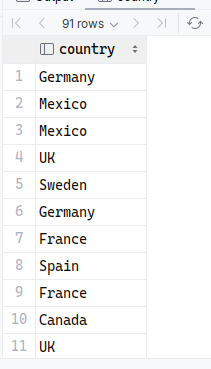
\includegraphics[height=6cm]{./images/p2-n1.png}
        \end{center}

        Karena data dari field \texttt{country} tidaklah unik untuk setiap record. Sehingga apabila kita melakukan seleksi pada field \texttt{country} saja,
        maka akan terlihat seolah olah data yg didapat merupakan duplikat dikarenakan field lain yang tidak terlihat.
    }
    \item {
        \begin{minted}[autogobble,fontsize=\small]{sql}
            SELECT DISTINCT country FROM Sales.Customers;
        \end{minted}

        Apakah ada data yang terduplikasi? Jelaskan perbedaan hasil pada lagkah tahap 4 dan
        tahap 3! Apa manfaat dari perintah \texttt{DISTINCT}? Capture hasil eksekusi script SQL diatas!

        \begin{center}
            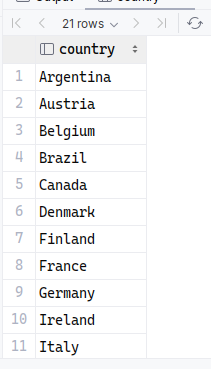
\includegraphics[height=6cm]{./images/p2-n2.png}
        \end{center}

        Tidak ada data yang terduplikasi. Perbedaan hasil pada tahap 4 dan 3 adalah pada tahap 4 kita melakukan seleksi pada field \texttt{country}
        menggunakan perintah \texttt{DISTINCT}. Perintah \texttt{DISTINCT} hanya akan mengembalikan hasil apabila data yang didapat unik.
    }
\end{enumerate}

\subsection{Part 5}
\begin{enumerate}
    \setcounter{enumi}{3}
    \item {
        \begin{minted}[autogobble,fontsize=\small]{sql}
            SELECT
                c.contactname, c.contacttitle
            FROM Sales.Customers AS c;

            SELECT
                c.contactname AS Name,
                c.contacttitle AS Title,
                c.companyname AS [Company Name]
            FROM Sales.Customers AS c;
        \end{minted}
        Apa yang membedakan hasil eksekusi dari query tahap 1 dan tahap 3 diatas? Apa
        manfaat dari perintah AS? Silahkan Jelaskan! Capture hasil eksekusi script SQL diatas!

        \begin{center}
            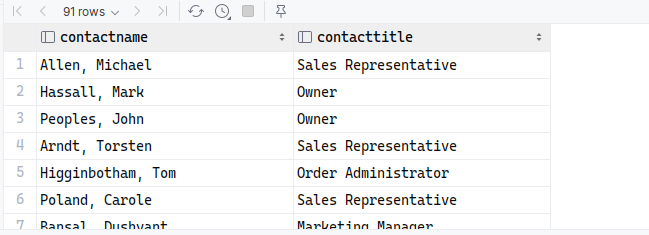
\includegraphics[height=3.5cm]{./images/p5.1-n1-a.png}\\
            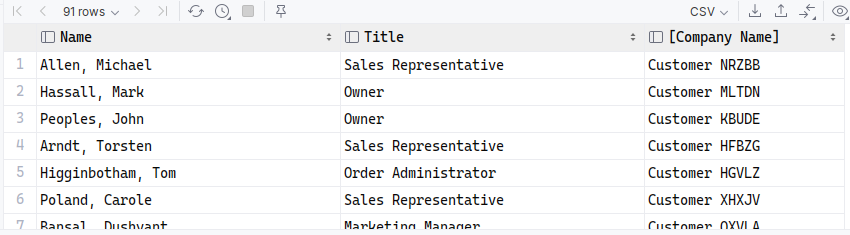
\includegraphics[height=3.5cm]{./images/p5.1-n1-b.png}\\
        \end{center}

        Perintah \texttt{AS} digunakan untuk memberikan alias pada field yang dipilih. Pada tahap 1 kita melakukan seleksi menggunakan
        tanpa menggunakan alias sehingga label tiap column akan mengikuti nama field pada tabel. Sedangkan pada tahap 3 kita memberikan alias
        pada tiap field yang dipilih sehingga label tiap column akan mengikuti alias yang diberikan.
    }
\end{enumerate}

\subsection{Part 4}
\begin{enumerate}
    \setcounter{enumi}{4}
    \item {
        \begin{minted}[autogobble,fontsize=\small]{sql}
            SELECT
                p.categoryid, p.productname
            FROM Production.Products AS p;

            SELECT
                p.categoryid,
                p.productname,
                CASE
                    WHEN p.categoryid = 1 THEN 'Beverages'
                    WHEN p.categoryid = 2 THEN 'Condiments'
                    WHEN p.categoryid = 3 THEN 'Confections'
                    WHEN p.categoryid = 4 THEN 'Dairy Products'
                    WHEN p.categoryid = 5 THEN 'Grains/Cereals'
                    WHEN p.categoryid = 6 THEN 'Meat/Poultry'
                    WHEN p.categoryid = 7 THEN 'Produce'
                    WHEN p.categoryid = 8 THEN 'Seafood'
                    ELSE 'Other'
                END AS categoryname
            FROM Production.Products AS p;
        \end{minted}

        \pagebreak

        Apa yang membedakan hasil eksekusi dari query tahap 1 dan tahap 3 diatas? Apa manfaat
        dari perintah CASE? Silahkan Jelaskan! Capture hasil eksekusi script SQL diatas

        \begin{center}
            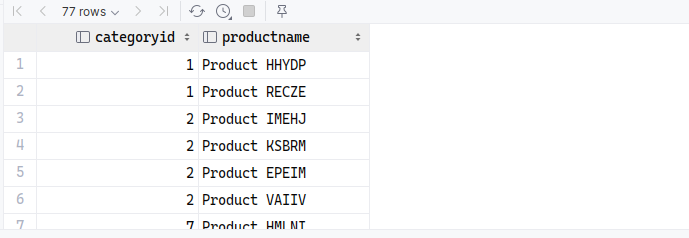
\includegraphics[height=4cm]{./images/p4-n1-a.png}\\
            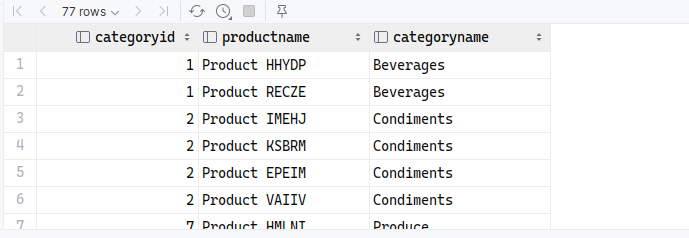
\includegraphics[height=4cm]{./images/p4-n1-b.png}
        \end{center}

        Pada tahap 1, query hanya melakukan seleksi pada field \texttt{categoryid} \\dan \texttt{productname}.
        Sedangkan pada tahap 3, query melakukan seleksi pada field yang sama dengan tambahan field baru yang diberi nama
        \texttt{categoryname}. Field ini merupakan hasil dari perintah \texttt{CASE} yang melakukan pengkondisian
        untuk mengubah angka menjadi teks berdasarkan value dari field \texttt{categoryid}
    }
    \item {
        \begin{minted}[fontsize=\small,autogobble]{sql}
            SELECT
                p.categoryid, p.productname,
                CASE
                    WHEN p.categoryid = 1 THEN 'Beverages'
                    WHEN p.categoryid = 2 THEN 'Condiments'
                    WHEN p.categoryid = 3 THEN 'Confections'
                    WHEN p.categoryid = 4 THEN 'Dairy Products'
                    WHEN p.categoryid = 5 THEN 'Grains/Cereals'
                    WHEN p.categoryid = 6 THEN 'Meat/Poultry'
                    WHEN p.categoryid = 7 THEN 'Produce'
                    WHEN p.categoryid = 8 THEN 'Seafood'
                    ELSE 'Other'
                END AS categoryname,
                CASE
                    WHEN p.categoryid IN (1, 7, 8) THEN 'Campaign Products'
                    ELSE 'Non-Campaign Products'
                END AS iscampaign
            FROM Production.Products AS p
        \end{minted}

        Silahkan capture hasilnya, data apa yang didapatkan dari perintah query diatas? Jelaskan!

        \begin{center}
            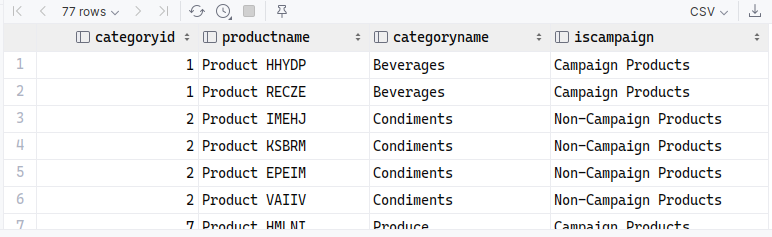
\includegraphics[height=4cm]{./images/p4-n2.png}\\
        \end{center}

        Pada tahap ini, query menambahkan field baru bernama \texttt{iscampaign} yang berisi data apakah produk tersebut merupakan
        produk yang sedang diiklankan atau tidak. Field ini merupakan hasil dari perintah \texttt{CASE} yang melakukan pengkondisian
        sama seperti pada tahap 5, namun alih alih mendefinisikan setiap kasus, kita menggunakan perintah \texttt{IN} untuk mendefinisikan
        beberapa kasus sekaligus, lalu mengabaikan sisanya menggunakan perintah \texttt{ELSE}.
    }
    \item {
        Capture perintah SQL anda dan berapa jumlah row yang dihasilkan!

        \begin{minted}[fontsize=\small,autogobble]{sql}
            SELECT
                p.categoryid AS ID_KATEGORI,
                p.productname AS NAMA_PRODUK,
                CASE
                    WHEN p.categoryid = 1 THEN 'Beverages'
                    WHEN p.categoryid = 2 THEN 'Condiments'
                    WHEN p.categoryid = 3 THEN 'Confections'
                    WHEN p.categoryid = 4 THEN 'Dairy Products'
                    WHEN p.categoryid = 5 THEN 'Grains/Cereals'
                    WHEN p.categoryid = 6 THEN 'Meat/Poultry'
                    WHEN p.categoryid = 7 THEN 'Produce'
                    WHEN p.categoryid = 8 THEN 'Seafood'
                    ELSE 'Other'
                END AS NAMA_KATEGORI,
                CASE
                    WHEN p.categoryid IN (1, 7, 8) THEN 'Campaign Products'
                    ELSE 'Non-Campaign Products'
                END AS STATUS
            FROM Production.Products AS p
            WHERE p.categoryid = 7;
        \end{minted}

        \begin{center}
            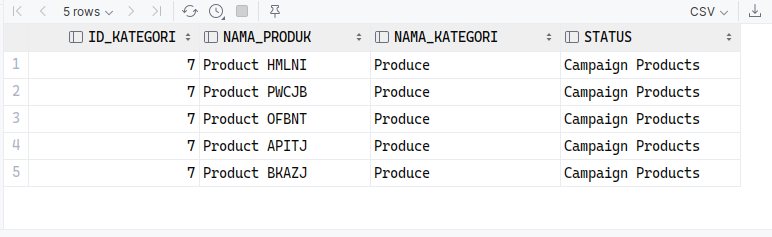
\includegraphics[height=4cm]{./images/p4-n3.png}
        \end{center}

        Terdapat 5 row yang dihasilkan dari query diatas.
    }
    \item {
        Tampilkan data employees dari tabel \texttt{HR.Employees} yang berasal dari negara `USA' dan kota
        `Seattle', gunakan perintah \texttt{ALIAS} untuk merubah nama kolom seperti gambar dibawah ini.
        Capture perintah SQL anda

        \begin{minted}[autogobble,fontsize=\small]{sql}
            SELECT
                e.firstname AS FIRST_NAME,
                e.lastname AS LAST_NAME,
                e.city AS CITY,
                e.country AS COUNTRY
            FROM HR.Employees AS e
            WHERE country = N'USA' AND city = N'Seattle';
        \end{minted}

        \begin{center}
            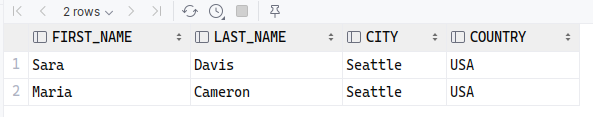
\includegraphics[height=2cm]{./images/p4-n4.png}
        \end{center}
    }
\end{enumerate}

\subsection{Part 5}
\begin{enumerate}
    \setcounter{enumi}{8}
    \item {
        Tulis perintah \texttt{SELECT} yang akan mengembalikan nilai pada kolom \texttt{custid}, \texttt{companyname},
        \texttt{contactname}, \texttt{address}, \texttt{city}, \texttt{country}, and \texttt{phone} pada tabel \texttt{Sales.Customers}, kemudian filter hasilnya
        hanya untuk ``Brazil, UK dan USA'' (Gunakan predikat \texttt{IN} dalam klausa \texttt{WHERE}).

        \begin{minted}[autogobble,fontsize=\small]{sql}
            SELECT
                c.custid,
                c.companyname,
                c.contactname,
                c.address,
                c.city,
                c.country,
                c.phone
            FROM Sales.Customers AS c
            WHERE country IN (N'Brazil', N'UK', N'USA');
        \end{minted}

        \begin{center}
            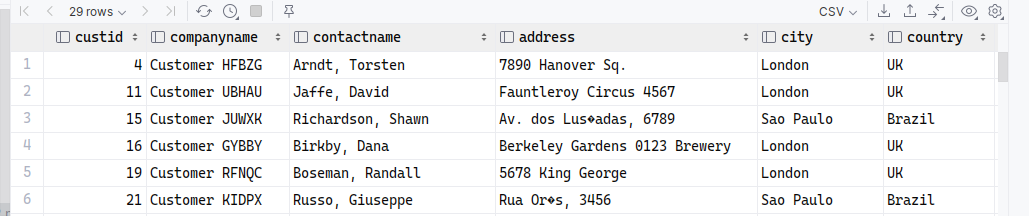
\includegraphics[height=2.8cm]{./images/p5-n1.png}
        \end{center}
    }
    \item {
        Salin Kode T-SQL pada tahap ke-4 kemudian modifikasi dengan operator perbandingan
        untuk kolom city pada clause \texttt{WHERE} dengan operator \texttt{OR}. Setelah itu eksekusi kode tersebut,
        tunjukkan hasilnya!

        \begin{minted}[autogobble,fontsize=\small]{sql}
            SELECT
                c.custid,
                c.companyname,
                o.orderid
            FROM Sales.Customers AS c
            LEFT OUTER JOIN Sales.Orders AS o 
                ON c.custid = o.custid OR c.city = 'Paris';
        \end{minted}

        \begin{center}
            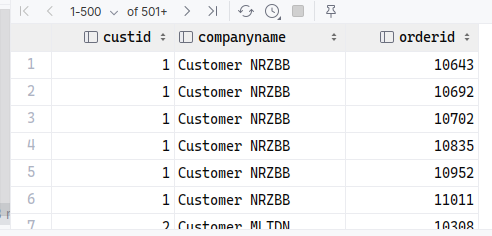
\includegraphics[height=4cm]{./images/p5-n2.png}
        \end{center}
    }
\end{enumerate}

\subsection{Part 6}
\begin{enumerate}
    \setcounter{enumi}{10}
    \item {
        Tuliskan perintah SELECT untuk mengambil kolom custid, custname dari tabel
        \texttt{Sales.Customers} dan kolom \texttt{orderid}, \texttt{orderdate} dari tabel \texttt{Sales.Orders}!
        Filter hasilnya hanya untuk pesanan pada atau setelah 1 April 2008.
        Kemudian urutkan hasilnya berdasarkan \texttt{orderdate} secara descending (menurun)
        dan \texttt{custid} ascending (menaik)!

        \begin{minted}[autogobble,fontsize=\small]{sql}
            SELECT
                c.custid,
                c.companyname,
                o.orderid,
                o.orderdate
            FROM Sales.Customers AS c
            INNER JOIN Sales.Orders AS o
                ON c.custid = o.custid
            WHERE o.orderdate >= '2008-04-01'
            ORDER BY o.orderdate DESC, c.custid ASC;
        \end{minted}

        \begin{center}
            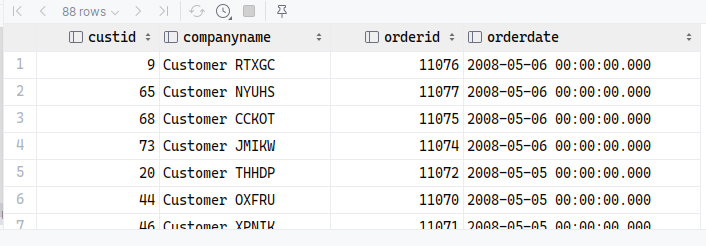
\includegraphics[height=4cm]{./images/p6-n1.png}
        \end{center}
    }
    \item {
        Eksekusi perintah T-SQL pada tahap 3. Apakah terjadi kesalahan?Apa pesan
        errornya? Menurut Anda, apakah penyebabnya?

        \begin{minted}[autogobble,fontsize=\small]{sql}
            SELECT
                e.empid, e.lastname, e.firstname, e.title, e.mgrid,
                m.lastname AS mgrlastname, m.firstname AS mgrfirstname
            FROM HR.Employees AS e
            INNER JOIN HR.Employees AS m ON e.mgrid = m.empid
            WHERE
            mgrlastname = N'Buck';
        \end{minted}

        Terjadi kesalahan dengan pesan error:

        \begin{minted}[fontsize=\small,autogobble]{sql}
            Invalid column name 'mgrlastname'.
        \end{minted}

        Hal ini disebabkan karena perintah \texttt{WHERE} tidak dapat mengakses field menggunakan alias.
    }
    \item {
        Lakukan perubahan perintah T-SQL untuk memperbaiki kesalahan pada uji coba ke-3,
        kemudian lakukan eksekusi! Bandingkan hasil eksekusi dengan hasil berikut. Jika sama, maka
        hasil uji coba sudah benar.

        \begin{minted}[autogobble,fontsize=\small]{sql}
            SELECT
                e.empid, e.lastname, e.firstname, e.title, e.mgrid,
                m.lastname AS mgrlastname, m.firstname AS mgrfirstname
            FROM HR.Employees AS e
            INNER JOIN HR.Employees AS m ON e.mgrid = m.empid
            WHERE
            e.mgrlastname = N'Buck';
        \end{minted}

        \begin{center}
            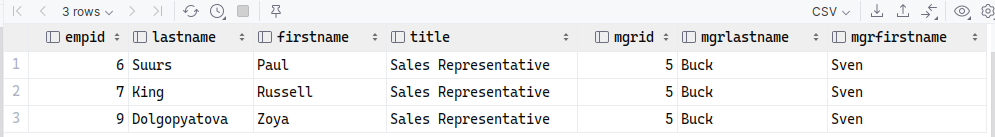
\includegraphics[height=1.85cm]{./images/p6-n3.png}
        \end{center}
    }
    \item {
        Salin perintah T-SQL pada uji coba 4, dan modifikasi sehingga menghasilkan semua
        karyawan \texttt{ORDER BY} nama depan manajer. Pada awalnya uji coba dengan menggunakan nama
        asal tabel, kemudian lakukan uji coba menggunakan nama alias tabel! Eksekusi T-SQL tersebut
        dan bandingkan dengan hasil berikut. Jika Hasilnya sama, maka uji coba sudah benar

        \begin{center}
            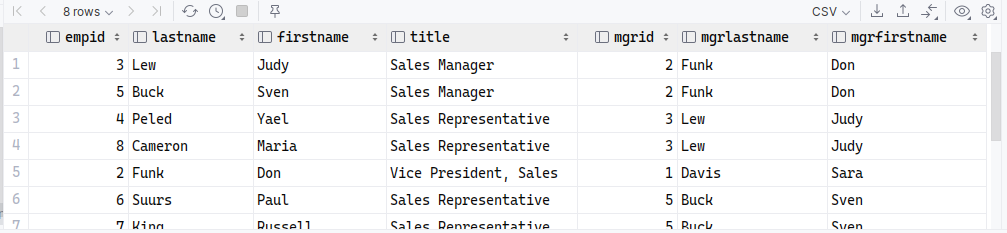
\includegraphics[height=2cm]{./images/p6-n4.png}
        \end{center}
    }
    \item {
        Kenapa kita dapat menggunakan nama kolom sesuai nama asli tabel ataupun
        menggunakan nama alias tabel?

        Karena nama alias tabel merupakan nama baru yang diberikan pada tabel yang digunakan untuk mempermudah
        penulisan query.
    }
\end{enumerate}

\subsection{Part 7}
\begin{enumerate}
    \setcounter{enumi}{15}
    \item {
        Tuliskan perintah \texttt{SELECT} untuk menampilkan kolom productname and\\ \texttt{unitprice} pada
        tabel \texttt{Production.Products} yang diurutkan secara menurun berdasarkan \texttt{unitprice}! Tampilkan
        hasil eksekusinya!

        \begin{minted}[autogobble,fontsize=\small]{sql}
            SELECT
                p.productname,
                p.unitprice
            FROM Production.Products As p
            ORDER BY unitprice DESC;
        \end{minted}

        \begin{center}
            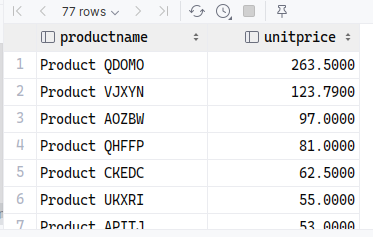
\includegraphics[height=4cm]{./images/p7-n1.png}
        \end{center}
    }
    \item {
        Salin dan modifikasi perintah T-SQL pada uji coba 2 dengan batasan hanya 8 produk
        yang akan ditampilkan berdasar pemesanan \texttt{unitprice}! Eksekusi perintah tersebut, dan
        bandingkan apakah sudah sesuai dengan hasil berikut.

        \begin{minted}[autogobble,fontsize=\small]{sql}
            SELECT TOP 8
                p.productname,
                p.unitprice
            FROM Production.Products As p
            ORDER BY unitprice DESC;
        \end{minted}

        \begin{center}
            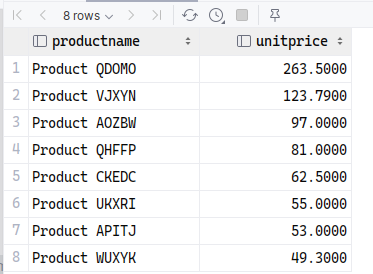
\includegraphics[height=5cm]{./images/p7-n2.png}
        \end{center}
    }
    \item {
        Apakah memungkinkan mengimplementasikan perintah T-SQL uji coba 5
        menggunakan klausa \texttt{OFFSET-FETCH}?

        \begin{minted}[autogobble,fontsize=\small]{sql}
            SELECT
                p.productname,
                p.unitprice
            FROM Production.Products As p
            ORDER BY unitprice DESC
            OFFSET 0 ROWS
            FETCH NEXT 8 ROWS ONLY;
        \end{minted}
    }
\end{enumerate}

\subsection{Part 8}
\begin{enumerate}
    \setcounter{enumi}{18}
    \item {
        Tuliskan perintah \texttt{SELECT} untuk menampilkan kolom \texttt{custid}, \texttt{orderid}, and \texttt{orderdate}
        pada tabel \texttt{Sales.Orders}. Urutkan baris berdasarkan \texttt{orderdate} dan \texttt{orderid}. Ambil 20 baris
        pertama. Eksekusi perintah tersebut dan bandingkan hasilnya berikut. Jika hasilnya sama, maka
        uji coba Anda sudah benar.

        \begin{minted}[fontsize=\small,autogobble]{sql}
            SELECT TOP 20
                custid,
                orderid,
                orderdate
            FROM Sales.Orders
            ORDER BY orderdate, orderid;
        \end{minted}

        \begin{center}
            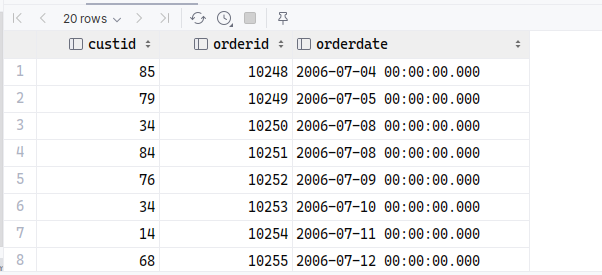
\includegraphics[height=4cm]{./images/p8-n1.png}
        \end{center}
    }
    \item {
        Tuliskan perintah \texttt{SELECT} untuk menampilkan hasil yang sama dengan soal no. 19,
        lewati 20 baris awal, dan lanjutkan dengan 20 baris selanjutnya menggunakan klausa \texttt{OFFSETFETCH}! Eksekusi perintah tersebut dan bandingkan dengan hasil berikut. Jika hasilnya sama,
        maka uji coba Anda sudah benar.

        \begin{minted}[fontsize=\small,autogobble]{sql}
            SELECT
                custid,
                orderid,
                orderdate
            FROM Sales.Orders
            ORDER BY orderdate, orderid
            OFFSET 20 ROWS
            FETCH NEXT 20 ROWS ONLY;
        \end{minted}

        \begin{center}
            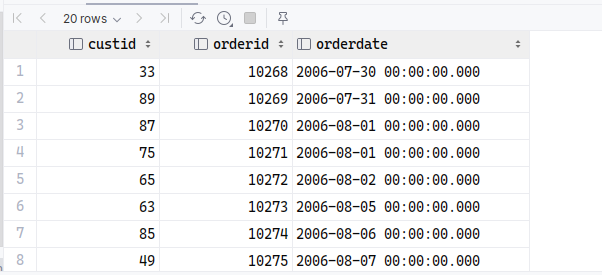
\includegraphics[height=4cm]{./images/p8-n2.png}
        \end{center}
    }
\end{enumerate}

\subsection{Part 9}
\begin{enumerate}
    \setcounter{enumi}{20}
    \item {
        Tulis sebuah SQL yang menampilkan hasil pada praktikum-1 langkah-1 \& 2 secara
        sekaligus (gabungan) dengan menggunakan \texttt{UNION}!

        \begin{minted}[autogobble,fontsize=\small]{sql}
            SELECT
                productid,
                productname
            FROM
                Production.Products
            WHERE categoryid = 4
            UNION
            SELECT
                P.productid,
                P.productname
            FROM Production.Products P
            INNER JOIN Sales.OrderDetails OD
                ON P.productid = OD.productid
            GROUP BY
                P.productid, P.productname
            HAVING SUM(OD.qty * OD.unitprice) > 50000;
        \end{minted}

        \begin{center}
            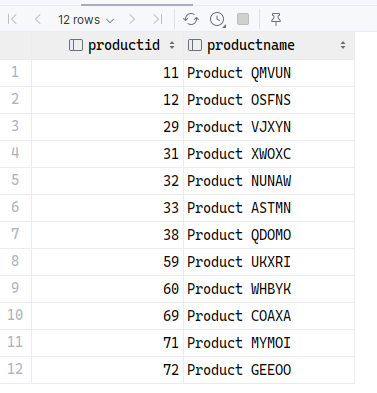
\includegraphics[height=6cm]{./images/p9-n1.png}
        \end{center}
    }
    \item {
        Serupa dengan langkah sebelumnya, kali ini tulislah sebuah SQL yang \\ menampilkan
        hasil pada praktikum-1 langkah-1 \& 2 secara sekaligus (gabungan) dengan menggunakan
        \texttt{UNION ALL}!

        \begin{minted}[autogobble,fontsize=\small]{sql}
            SELECT
                productid,
                productname
            FROM
                Production.Products
            WHERE categoryid = 4
            UNION ALL
            SELECT
                P.productid,
                P.productname
            FROM Production.Products P
            INNER JOIN Sales.OrderDetails OD
                ON P.productid = OD.productid
            GROUP BY
                P.productid, P.productname
            HAVING SUM(OD.qty * OD.unitprice) > 50000;
        \end{minted}

        \begin{center}
            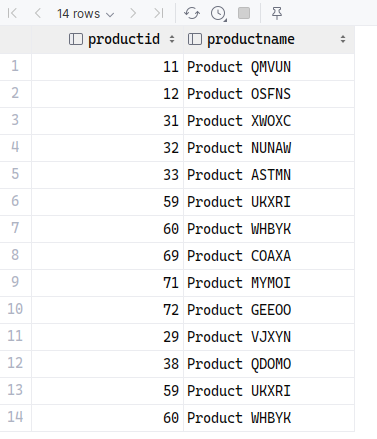
\includegraphics[height=6cm]{./images/p9-n2.png}
        \end{center}
    }
    \item {
        Apa bedanya \texttt{UNION} \& \texttt{UNION ALL}?

        \begin{itemize}
            \item \textbf{UNION:} Hanya mengembalikan record yang memiliki nilai unik
            \item \textbf{UNION ALL:} Mengembalikan keseluruhan record tanpa mempedulikan hasil yang duplikat
        \end{itemize}
    }
    \item {
        Tuliskan SQL untuk menampilkan 10 pelanggan yang membeli paling awal serta 10
        pelanggan yang membeli paling akhir.

        \begin{minted}[autogobble,fontsize=\small]{sql}
            SELECT TOP 10
                c.custid,
                c.companyname,
                o.orderdate
            FROM Sales.Customers AS c
            INNER JOIN Sales.Orders AS o
                ON c.custid = o.custid
            ORDER BY o.orderdate DESC;

            SELECT TOP 10
                c.custid,
                c.companyname,
                o.orderdate
            FROM Sales.Customers AS c
            INNER JOIN Sales.Orders AS o
                ON c.custid = o.custid
            ORDER BY o.orderdate ASC;
        \end{minted}
    }
\end{enumerate}

\end{document}

